\chapter{Etude du format PE}

\section{Introduction au format Portable Executable}
Le format PE (Portable Executable), est un format du fichier natif spécifique à Microsoft Windows, qui structure les fichiers exécutable du système d'exploitation. Développé par Microsoft, et dérivé d'Unix COFF (Common Object File Format), ce format structure les binaires à extension *.exe (Logiciel), *.ocx (Object Linking and Embbeding), *.dll (Dynamic Link Library) et *.cpl (Panneau de Configuration) sur toutes les plateformes Win32 et supérieur~\cite{wiki}.
\\

D'un point de vue sécuritaire, la connaissance de ce format est en soit une base qu'il est nécessaire de posséder lorsque l'on souhaite se lancer dans la conception et développement d'un parseur de PE.
\section{Bref historique}
Microsoft migra vers le format PE avec l'introduction de Microsoft Windows NT 3.1. Toutes les versions suivantes de Microsoft Windows, incluant Microsoft Windows 95/98/ME, supportent ce format. Auparavant les fichiers avec \og exécutable \fg. étaient au format NE \og Executable File Format \fg.\\
 La création du format PE a été induite par le fait que Microsoft souhaitait créer une structure du fichier portable, de sorte qu'elle puisse s'adapter aux différents systèmes de Microsoft Windows NT, car il faut savoir que Microsoft Windows NT était au départ capable de supporter d'autres architectures que le x86 d'Intel, Power PC et Motorola 68000 en faisaient partie~\cite{MS}.
\\
L'idée fût donc de créer une structure commune à ces architectures.
\section{Schéma du format PE}
PE étant une structure du fichier, cela signifie qu'il est formaté d'une certaine façon. La figure~\ref{fig :PEX} montre son formatage :
\begin{figure}[H]
\begin{center}
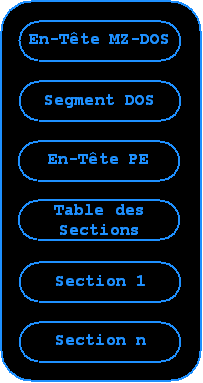
\includegraphics[scale=0.6]{Figures/PE.png}
\caption{Organisation générale d'un fichier PE}
\label{fig :PEX} 
\end{center}
\end{figure}

Tous les fichiers PE respectent ce formatage. Si on essaye, par exemple, d'ouvrir un fichier *.exe avec un éditeur hexadécimal on s'aperçoit que les deux premiers octets sont MZ, qui correspondent bien aux 2 premiers octets de l'en-tête MZ-DOS décrit ci-dessous.
\subsection{En-tête MZ-DOS}
L'en-tête MZ-DOS permet au système d'exploitation de reconnaître le fichier comme étant un exécutable valide dans le cas où celui-ci serait lancé depuis MS-DOS,afin de pouvoir exécuter son segment DOS. Cet en-tête est également soumis à une structuration, nommée IMAGE\_DOS\_HEADER, cette structure permet de formater l'en-tête MZ-DOS. Ci-dessous, son prototype en langage C.
\begin{lstlisting}
typedef struct _IMAGE_DOS_HEADER { // DOS .EXE header
WORD e_magic;                      // Magic number
WORD e_cblp;                       // Bytes on last page of file
WORD e_cp;                         // Pages in file
WORD e_crlc;                       // Relocations
WORD e_cparhdr;                    // Size of header in paragraphs
WORD e_minalloc;                   // Minimum extra paragraphs needed
WORD e_maxalloc;                   // Maximum extra paragraphs needed
WORD e_ss;                         // Initial (relative) SS value
WORD e_sp;                         // Initial SP value
WORD e_csum;                       // Checksum
WORD e_ip;                         // Initial IP value
WORD e_cs;                         // Initial (relative) CS value
WORD e_lfarlc;                     // File address of relocation table
WORD e_ovno;                       // Overlay number
WORD e_res[4];                     // Reserved words 
WORD e_oemid;                      // OEM identifier (for e_oeminfo)
WORD e_oeminfo;                    // OEM information; e_oemid specific
WORD e_res2[10];                   // Reserved words
LONG e_lfanew;                     // File address of new exe header
} IMAGE_DOS_HEADER, *PIMAGE_DOS_HEADER;
\end{lstlisting}
\newpage
La figure~\ref{fig :pic1} montre un exemple réel avec le parseur CFF Explorer :
\begin{figure}[H]
\begin{center}
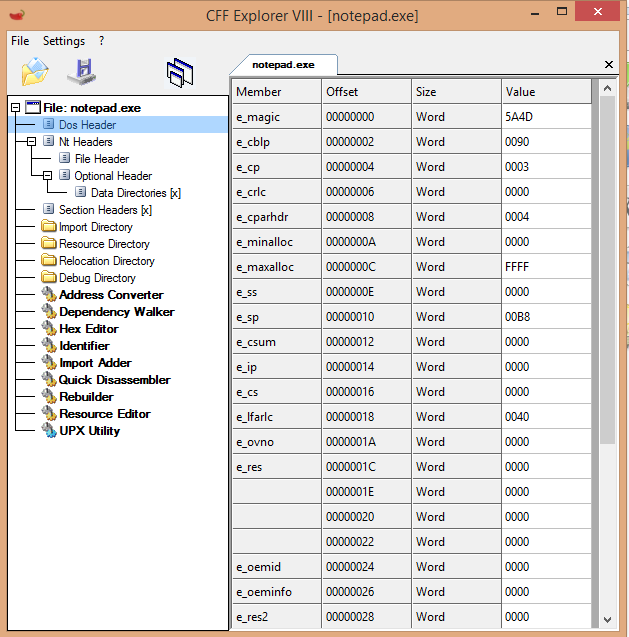
\includegraphics[scale=0.7]{Figures/pic1.PNG}
\caption{ En-tête MZ-DOS d'un fichier PE avec CFF Explorer.}
\label{fig :pic1} 
\end{center}
\end{figure}
les champs les plus importants sont :
\begin{itemize}
\item \textbf{e\_magic : }qui doit valoir "MZ"
\item \textbf{e\_lfanew : }contient l'adresse du début de l'en-tête PE.
\end{itemize}
\subsection{Segment DOS}
Le segment DOS est exécuté lorsque l'application est lancée sous MS-DOS au lieu d'un environnement fenêtré Microsoft Windows, il affiche en général un message comme "This program must be run under Win32", autrement dit "Ce programme doit être exécuté sous Win32". Il s'agit d'un message implémenté par le compilateur, lors de la compilation du code logiciel, et dans le plupart des cas une exécution de int 21h, une interruption du BIOS (Basic Input Ouput System) qui permet d'afficher un texte à l'écran.\\


La figure~\ref{fig :pic2} montre l'ouverture d'un fichier PE avec éditeur hexadécimal.
\begin{figure}[H]
\begin{center}
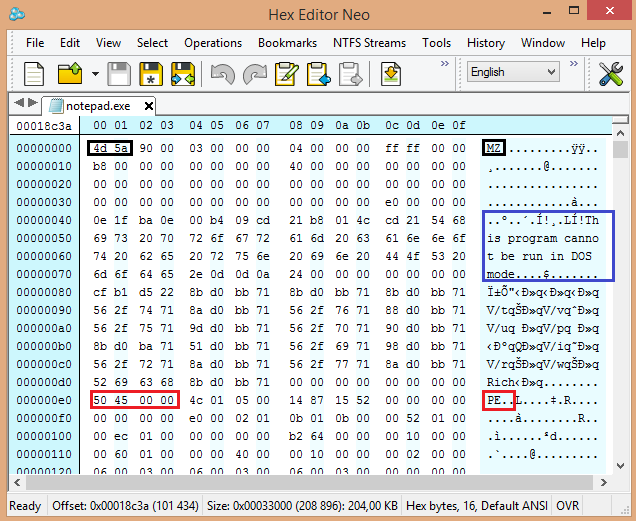
\includegraphics[scale=0.8]{Figures/pic2.PNG}
\caption{ Segment DOS d'un fichier PE avec Hex Editor.}
\label{fig :pic2} 
\end{center}
\end{figure}
\subsection{En-tête PE}
L'en-tête PE est un ensemble de structures, regroupées dans une même et unique nommé IMAGE\_NT\_HEADER,
voici son prototype en langage C.
\begin{lstlisting}
typedef struct _IMAGE_NT_HEADERS {
DWORD                 Signature;
IMAGE_FILE_HEADER     FileHeader;
IMAGE_OPTIONAL_HEADER OptionalHeader;
}IMAGE_NT_HEADERS, *PIMAGE_NT_HEADERS;
\end{lstlisting}


Le premier champ,\textbf{Signature : }signature Signature permettant d'identifier le fichier, qui doit être égale à 0x00004550, soit "PE00". (voire la figure~\ref{fig :pic2} qui est en rouge).
\\
\subsection{L'en-tête du fichier}

L'en-tête du fichier est une structure nommé IMAGE\_FILE\_HEADER, qui contient les informations
concernant la structuration du fichier. Elle est prototypée comme suit :
\begin{lstlisting}
typedef struct _IMAGE_FILE_HEADER {
WORD   Machine;                       
WORD   NumberOfSections;
DWORD  TimeDateStamp;
DWORD  PointerToSymbolTable;
DWORD  NumberOfSymbols;
WORD   SizeOfOptionalHeader;
WORD   Characteristics;
}IMAGE_FILE_HEADER, *PIMAGE_FILE_HEADER;
\end{lstlisting}
Le Tableau~\ref{tab1} explique les champs de la structure IMAGE\_FILE\_HEADER:
\begin{table}[h]
\begin{tabular}{|p{4.5cm}|p{10.5cm}|}
\hline \textbf{champ} &  \textbf{contenu}\\
\hline Machine & Le processeur pour lequel le fichier est prévu.\\
\hline NumberOfSections & Le nombre de sections dans le fichier.\\
\hline TimeDateStamp & La date et l'heure auxquelles le fichier a été créé.\\
\hline PointerToSymbolTable & Utilisé pour le débogage. Semble être toujours 0.\\
\hline NumberOfSymbols & Utilisé pour le débogage. Semble être toujours 0.\\
\hline SizeOfOptionalHeader & Taille de la structure OptionalHeader.\\
\hline Characteristics & Contient des flags pour le fichier.\\
\hline
\end{tabular}
\caption{La structure de l'en-tête du fichier PE}
\label{tab1}
\end{table}
Exemple réel avec CFF Explorer (figure~\ref{fig :pic3} ) :
\begin{figure}[H]
\begin{center}
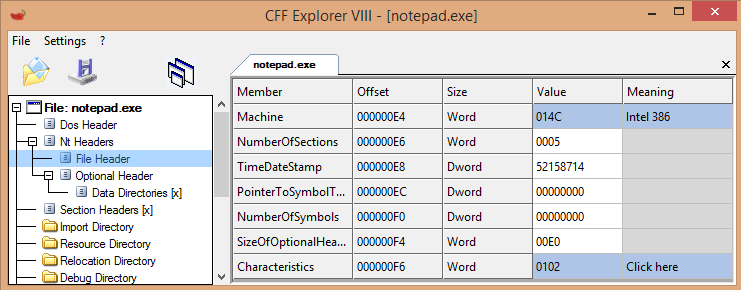
\includegraphics[scale=0.7]{Figures/pic3.PNG}
\caption{ L'en-tête du fichier PE avec CFF Explorer.}
\label{fig :pic3} 
\end{center}
\end{figure}

\subsection{L'en-tête facultatif}

L'en-tête facultatif est le dernier membre de la structure IMAGE\_NT\_HEADER. Il contient des informations sur l'organisation logique du fichier PE~\cite{PE}.
Il est prototypé comme suit :
\begin{lstlisting}

typedef struct _IMAGE_OPTIONAL_HEADER {
  WORD                 Magic;
  BYTE                 MajorLinkerVersion;
  BYTE                 MinorLinkerVersion;
  DWORD                SizeOfCode;
  DWORD                SizeOfInitializedData;
  DWORD                SizeOfUninitializedData;
  DWORD                AddressOfEntryPoint;
  DWORD                BaseOfCode;
  DWORD                BaseOfData;
  DWORD                ImageBase;
  DWORD                SectionAlignment;
  DWORD                FileAlignment;
  WORD                 MajorOperatingSystemVersion;
  WORD                 MinorOperatingSystemVersion;
  WORD                 MajorImageVersion;
  WORD                 MinorImageVersion;
  WORD                 MajorSubsystemVersion;
  WORD                 MinorSubsystemVersion;
  DWORD                Win32VersionValue;
  DWORD                SizeOfImage;
  DWORD                SizeOfHeaders;
  DWORD                CheckSum;
  WORD                 Subsystem;
  WORD                 DllCharacteristics;
  DWORD                SizeOfStackReserve;
  DWORD                SizeOfStackCommit;
  DWORD                SizeOfHeapReserve;
  DWORD                SizeOfHeapCommit;
  DWORD                LoaderFlags;
  DWORD                NumberOfRvaAndSizes;
  IMAGE_DATA_DIRECTORY DataDirectory[IMAGE_NUMBEROF_DIRECTORY_ENTRIES];
} IMAGE_OPTIONAL_HEADER, *PIMAGE_OPTIONAL_HEADER;
\end{lstlisting}


Cette structure comporte 31 champs. Certains d'entre eux sont cruciaux et d'autres ne sont pas utiles. Nous verrons uniquement les champs qui sont réellement utiles.\\
Exemple réel avec CFF Explorer (voire figure~\ref{fig :pic4}) :
\begin{figure}[H]
\begin{center}
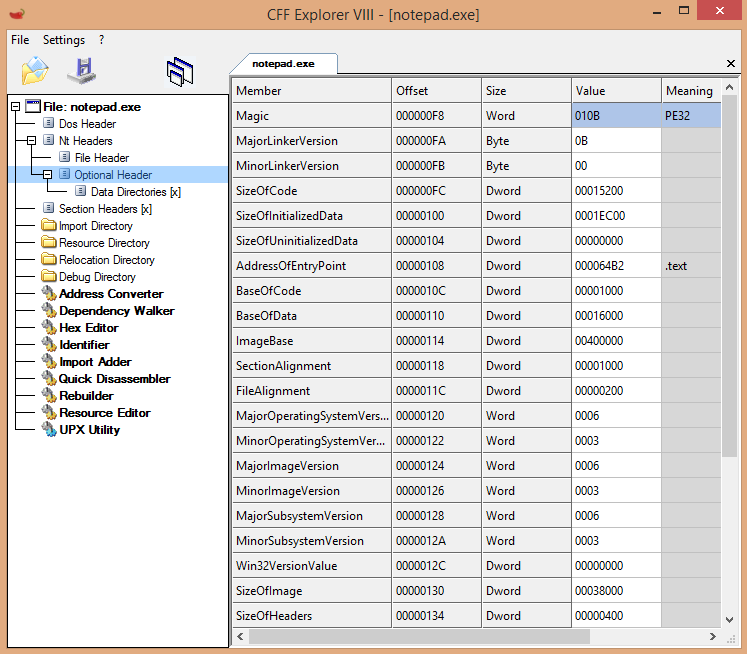
\includegraphics[scale=0.7]{Figures/pic4.PNG}
\caption{ L'en-tête facultatif d'un fichier PE avec CFF Explorer.}
\label{fig :pic4} 
\end{center}
\end{figure}


Un mot revient fréquemment en relation avec le format PE : \textbf{RVA}.\\
RVA signifie Relative Virtual Address. RVA est un terme un peu rebutant pour un concept aussi simple. Pour parler simplement, une RVA est une distance à partir d'un point de référence dans l'espace d'adressage virtuel. Une RVA est exactement la même chose qu'un offset fichier. Toutefois, elle est relative à une adresse virtuelle plutôt qu'au début d'un fichier.\\
Voici un exemple :\\
Si un fichier PE est chargé à l'adresse \$400000 dans l'espace d'adressage virtuel et que le programme commence son exécution à l'adresse \$401000, on peut dire que le programme débute à la RVA \$1000. Une RVA est relative à l'adresse virtuelle du premier octet du module.\\
Pourquoi le format PE utilise-t-il des RVA ? Le but est de réduire le temps de chargement du PE Loader. Sachant qu'un module peut être déplacé n'importe où dans l'espace d'adressage virtuel, ce serait infernal pour le PE Loader de fixer les adresses de chaque élément à position variable du module. Par opposition, si tous les éléments ayant une position variable dans le fichier utilisent des RVA, le PE Loader n'a alors pas besoin de fixer quoi que ce soit : il déplace simplement tout le module à une nouvelle adresse virtuelle. Tout cela rejoint le concept de chemin relatif et chemin absolu : une RVA est assimilable à un chemin relatif, une adresse virtuelle à un chemin absolu.\\

Voici le tableau~\ref{tab2} qui donne les champs intéressants de l'en-tête facultatif : 

\begin{table}[h]
\begin{tabular}{|p{4.5cm}|p{11cm}|}
\hline \textbf{champ} &  \textbf{contenu}\\
\hline AddressOfEntryPoint & Il s'agit de la RVA de la première instruction qui sera exécutée lorsque le PE Loader sera prêt à lancer le fichier.\\
\hline ImageBase &	C'est l'adresse de chargement souhaitable pour le fichier PE.\\
\hline SectionAlignment & La granularité de l'alignement des sections en mémoire.\\
\hline FileAlignment & La granularité de l'alignement des sections dans le fichier.\\
\hline MajorSubSystemVersion & La version du système Win32.\\
\hline MinorSubSystemVersion & La version du système Win32.\\
\hline SizeOfImage & La taille totale du fichier PE en mémoire. C'est la somme de tous les en-têtes et des sections alignées avec la valeur SectionAlignment.\\
\hline SizeOfHeaders & La taille de tous les en-têtes et de la table des sections. Cette valeur est égale à la taille du fichier moins la taille de toutes les sections.\\
\hline Subsystem & Donne pour quel sous-système NT le fichier PE est prévu.\\
\hline DataDirectory & Un tableau de structures IMAGE\_DATA\_DIRECTORY.\\
\hline

\end{tabular}
\caption{Les champs intéressants de l'en-tête facultatif}
\label{tab2}
\end{table}
\subsection{Table des Sections}
La table des sections est en fait un tableau de structures suivant immédiatement l'en-tête PE. Le nombre de membres dans ce tableau est donné par le champ NumberOfSections dans l'en-tête fichier (IMAGE\_FILE\_HEADER). La structure en question est appelée IMAGE\_SECTION\_HEADER. La Table des Sections est prototypée comme suit :
\begin{lstlisting}
typedef struct _IMAGE_SECTION_HEADER {

BYTE Name[IMAGE_SIZEOF_SHORT_NAME];
union {
DWORD PhysicalAddress;
DWORD VirtualSize;
} Misc;
DWORD VirtualAddress;
DWORD SizeOfRawData;
DWORD PointerToRawData;
DWORD PointerToRelocations;
DWORD PointerToLinenumbers;
WORD NumberOfRelocations;
WORD NumberOfLinenumbers;
DWORD Characteristics;

} IMAGE_SECTION_HEADER, *PIMAGE_SECTION_HEADER;

\end{lstlisting}
La figure~\ref{fig :pic6} montre la table des sections d'un fichier PE avec CFF Explorer :
\begin{figure}[H]
\begin{center}
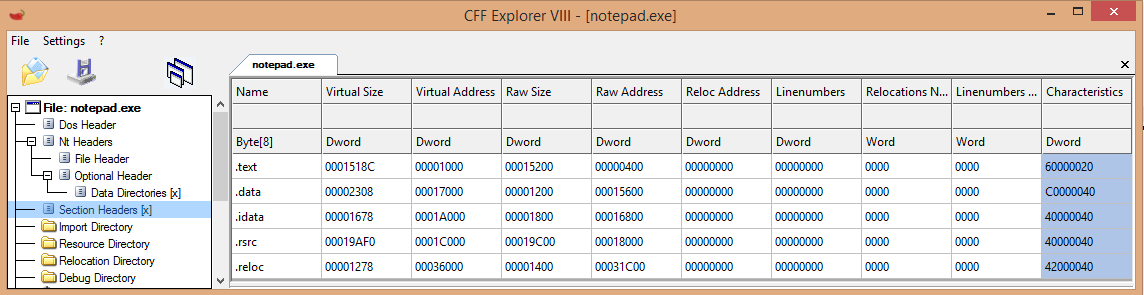
\includegraphics[scale=0.5]{Figures/pic6.PNG}
\caption{ La table des sections d'un fichier PE avec CFF Explorer.}
\label{fig :pic6} 
\end{center}
\end{figure}


le tableau~\ref{tab3} explique les champs qui sont vraiment intéressants : 
\begin{table}[H]
\begin{tabular}{|p{4.5cm}|p{10.5cm}|}
\hline \textbf{champ} &  \textbf{contenu}\\
\hline Name & Ce champ contient le nom de la section, il est là seulement à titre informatif pour le programmeur.\\
\hline VirtualAddress &	La RVA de la section. Le PE Loader vérifie et utilise la valeur de ce champ lorsqu'il place une section en mémoire.\\
\hline SizeOfRawData & La taille des données de la section, arrondie au prochain multiple de FileAlignment. Le PE Loader vérifie ce champ pour savoir combien d'octets de la section il va devoir placer en mémoire.\\
\hline PointerToRawData & L'offset fichier du début de la section. Le PE Loader utilise la valeur de ce champ pour trouver les données de la section dans le fichier.\\
\hline Characteristics & Contient des drapeaux indiquant par exemple si la section contient du code exécutable, des données non initialisées, si elle dispose d'un accès en écriture ou en lecture.\\
\hline
\end{tabular}
\caption{La structure de Table des Sections}
\label{tab3}
\end{table}


Chaque fichier PE contient un ensemble de sections, définit dans la Table des Sections. Une section est en fait un "segment" du fichier, possédant certaines particularités. Ci-dessous, Le tableau~\ref{tab4} montre
les différentes sections existantes.
\begin{table}[H]
\begin{tabular}{|p{2 cm}|p{12 cm}|}
\hline \textbf{Nom} &  \textbf{Description}\\
\hline .text & Généralement le code (instructions) du programmme.\\
\hline .bss & Contient des données non-initialisées.\\
\hline .reloc & Relocation.\\
\hline .data & Contient des données initialisées.\\
\hline .rsrc & Généralement les ressources du fichier (Curseurs, Sons, Menus ...)\\
\hline .rdata & Contient l'IAT d'un fichier.\\
\hline .idata & Contient l'IAT d'un fichier.\\
\hline .upx & Signe d'une compression UPX, propre au logiciel UPX.\\
\hline .aspack & Signe d'un package ASPACK, propre au logiciel ASPACK.\\
\hline .adata & Signe d'un package ASPACK, propre au logiciel ASPACK.\\
\hline
\end{tabular}
\caption{ Sections des fichiers PE}
\label{tab4}
\end{table}
La figure~\ref{fig :pic5} montre la table des sections d'un fichier PE avec éditeur hexadécimal :
\begin{figure}[H]
\begin{center}
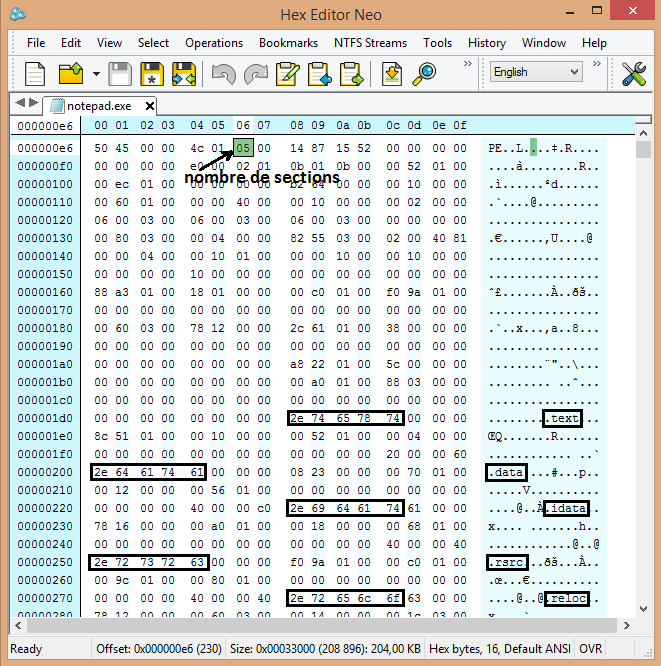
\includegraphics[scale=0.8]{Figures/pic5.PNG}
\caption{ La table des sections d'un fichier PE avec Hex Editor.}
\label{fig :pic5} 
\end{center}
\end{figure} 
\subsection{La table d'importation}
L'IAT, qui signifie \textbf{Import Address Table}, est une section (.idata ou .rdata) contenant les adresses des API importées par un logiciel, ainsi que les noms des DLL exportant ces fonctions. Les API, exportées par ces DLL, permettent aux logiciels de fonctionner correctement. Son existence est dû au fait que les API sont adressées différemment en fonction des OS.\\
La section \textbf{.idata} (ou \textbf{.rdata} parfois), qui contient cette IAT, est formaté d'une certaine façon. Il faut savoir en premier lieu qu'une structure nommée "ImageImportDescriptor" est utilisé pour chaque DLL appelée; plus une dernière de 5 DWORD mise à zéro qui définit une terminaison.\\
Pour chaque DLL importée, une structure nommée IMAGE\_THUNK\_DATA sera utilisée pour chaque API de cette
DLL; il y aura donc autant de IMAGE\_THUNK\_DATA que de fonctions exportées par une DLL, plus un dernier
DWORD spécifiant la terminaison de cette DLL. Une troisième structure, IMAGE\_IMPORT\_BY\_NAME, définit le nom des API ainsi que leur numéro ORDINAL (Nombre de 16 bits identifiant une fonction au sein d'une DLL). Il en existe autant qu'il y a d'API importées par DLL.
Par exemple, sur l'image~\ref{fig :IAT} d'exemple ci-dessous, il y a trois IMAGE\_IMPORT\_BY\_NAME définis pour user32.dll, car seulement trois de ses API sont utilisées par le programme.
\begin{figure}[H]
\begin{center}
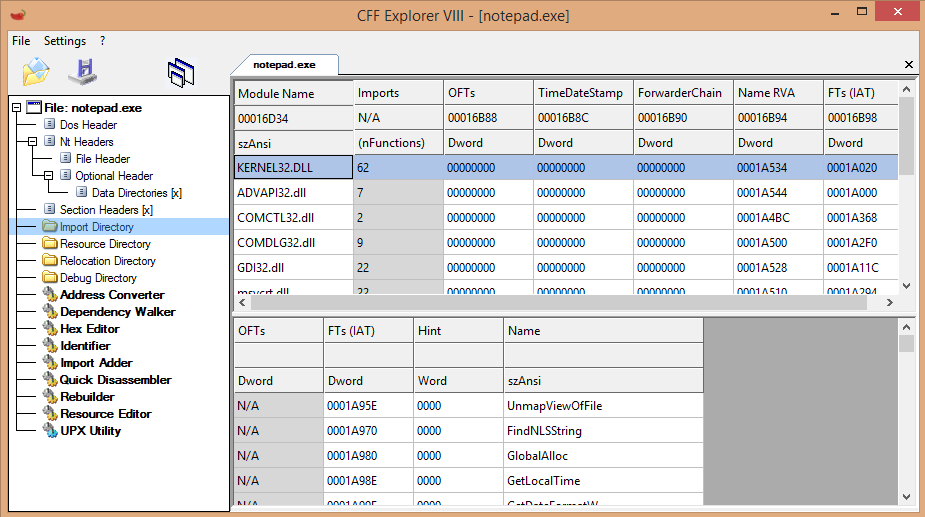
\includegraphics[scale=0.6]{Figures/pic7.PNG}
\caption{Table d'importation d'un fichier PE}
\label{fig :IAT} 
\end{center}
\end{figure}
La Table d'importation est prototypée comme suit :
\begin{lstlisting}

typedef struct _IMAGE_IMPORT_DESCRIPTOR {

DWORD Characteristics; 
DWORD OriginalFirstThunk; 
DWORD TimeDateStamp; 
DWORD ForwarderChain; 
DWORD Name; 
DWORD FirstThunk; 

} IMAGE_IMPORT_DESCRIPTOR;

typedef struct _IMAGE_IMPORT_BY_NAME {

WORD Hint; //Ordinal Number
BYTE Name[1]; //Name of function

} IMAGE_IMPORT_BY_NAME, *PIMAGE_IMPORT_BY_NAME;

typedef struct _IMAGE_THUNK_DATA {

PDWORD Function;
PIMAGE_IMPORT_BY_NAME AddressOfData;

} IMAGE_THUNK_DATA, *PIMAGE_THUNK_DATA;
\end{lstlisting}
\subsection{La table d'exportation}
Quand le PE Loader exécute un programme, il charge les DLL associées dans l'espace d'adressage du processus. Il extrait ensuite les informations des fonctions importées à partir du programme principal. Il utilise ces informations pour rechercher les adresses de ces fonctions dans les DLL, afin de les renseigner dans le code du processus. L'endroit où le PE Loader cherchera ces adresses se trouve être la table d'exportation de ces mêmes DLL.\\
Il existe deux manières pour une DLL ou un EXE d'exporter une fonction afin de la rendre utilisable par un programme externe : elle peut être exportée par nom, ou uniquement par ordinal.\\
Comme pour la table d'importation, la localisation de la table d'exportation peut être retrouvée dans le data directory. Ici, la table d'exportation en est le premier membre. La structure d'exportation est appelée IMAGE\_EXPORT\_DIRECTORY. Elle est prototypée comme suit :
\begin{lstlisting}
typedef struct _IMAGE_EXPORT_DIRECTORY {

DWORD  Characteristics;           /* 0x00 */
DWORD  TimeDateStamp;             /* 0x04 */
WORD   MajorVersion;              /* 0x08 */
WORD   MinorVersion;              /* 0x0a */
DWORD  Name;                      /* 0x0c */
DWORD  Base;                      /* 0x10 */
DWORD  NumberOfFunctions;         /* 0x14 */
DWORD  NumberOfNames;             /* 0x18 */
DWORD  AddressOfFunctions;        // 0x1c RVA from base of image
DWORD  AddressOfNames;            // 0x20 RVA from base of image
DWORD  AddressOfNameOrdinals;     // 0x24 RVA from base of image

} IMAGE_EXPORT_DIRECTORY, *PIMAGE_EXPORT_DIRECTORY;
\end{lstlisting}
\section{Le PE Loader}
Le PE Loader est un élément de Microsoft Windows permettant de reconnaître et de charger en mémoire des fichiers PE. C'est grâce à lui que Microsoft Windows peut exécuter les instructions d'un tel fichier.\\


Voici son fonctionnement global :
\begin{itemize}
\item Le PE Loader examine l'en-tête MZ-DOS afin de trouver l'offset de l'en-tête PE. S'il le trouve il saute dessus
\item Il vérifie la validité de l'en-tête PE. Si tel est le cas il saute à la fin de cet en-tête
\item Il lit les informations concernant les sections puis mappe ces sections en mémoire en employant un procédé de "File Mapping" (copie d'un fichier en mémoire).

\end{itemize}
        
\section{Les Packers}
Un Packer est un utilitaire dont le but est de compresser un programme afin de réduire sa taille initiale, tout en conservant son aspect exécutable ( le code original est retrouvé en mémoire lors de l'extraction ).\\
Néanmoins, avec le temps, des nouveaux packers sont apparus et ces derniers possèdent également la capacité de chiffrer le code du programme cible, ce qui aura pour effet de réduire son poids certes, mais qui de plus, va modifier son code d'exécution. Un algorithme des plus connu, et un des plus simple à contourner (clé généralement en dur dans le programme), est sans nul doute XOR (OU-Exclusif).\\
Bien entendu, la partie "déchiffrement" effectué lors du lancement du programme packé/chiffré sera établie de manière transparente pour l'utilisateur. Mais un désassembleur  verra cela autrement, en visualisant un code (très) différent de la normale.\\

Les cybercriminels ont recours aux packers pour eviter que l'antivirus puisse identifier le malware rapidement. le meme malware (même identifié par l'antivirus) lorsqu'il est packé, la signature ne matchera pas et il ne sera pas détecté. mais comme les antivirus ont du mal a analyser les malwares en mémoire (lorsqu'ils sont dépackés), alors les packers sont une bonne protection pour les cybercriminels. Aussi, ils servent à ralentir les analystes dans l'analyse de malware car ils intégrant des méthodes d'antidebug, antivm, et autres.
un packer malveillant peut identifier qu'il est exécuté dans une virtuel machine, qu'il est analysé avec un debugger, ...\\

Il existe de nombreux packers tel que : Armadillo, ASPack \& ASProtect, NeoLite, PKLite, Petite v1.4/2.x, PolyCrypt PE, Shrinker, VBox, WWPack(32), ...\\

Un des Packers sans nul doute le plus connu est UPX, qui s'occupe de réduire la taille d'un exécutable de manière très efficace (près de 50\%). La figure~\ref{fig :UPX} montre le packer UPX.
\begin{figure}[H]
\begin{center}
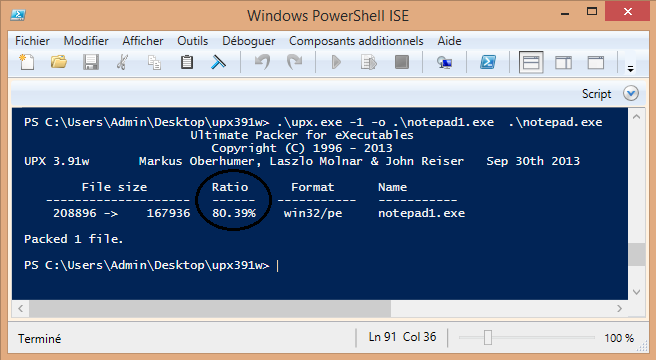
\includegraphics[scale=0.7]{Figures/UPX.png}
\caption{Le Packer UPX}
\label{fig :UPX} 
\end{center}
\end{figure}
Lorsque le programme packé est exécuté, un chargeur/décompresseur (wrapper program) est exécuté aussi pour décompresser le fichier packé puis exécuter le fichier décompressé, comme le montre la figure~\ref{fig :PACK}. Quand un  programme packé est analysé statiquement, seul le chargeur/décompresseur peut être disséqué~\cite{ANA}.
\begin{figure}[H]
\begin{center}
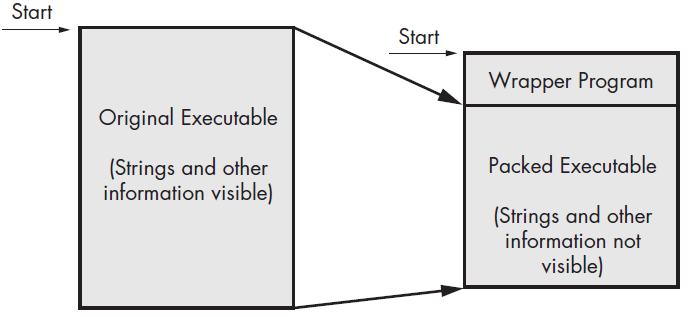
\includegraphics[scale=0.6]{Figures/PACK.png}
\caption{Fichier original et fichier packé}
\label{fig :PACK} 
\end{center}
\end{figure}
\subsection{Détection des Packers avec PEiD}
Une façon de détecter des fichiers compressés (packés) est avec le programme PEiD. Il est possible d'utiliser PEiD pour détecter le type de packer ou le compilateur utilisé pour construire une application, ce qui rend l'identification d'un fichier packé, avec un packer connu, beaucoup plus facile.\\
PEiD contient une base de signature permettant d'identifier les packers/compilateurs utilisés, cette base s'appelle UpdateDB.txt.
 La figure~\ref{fig :PEID} montre l'analyse d'un fichier .exe par PEiD.
\begin{figure}[H]
\begin{center}
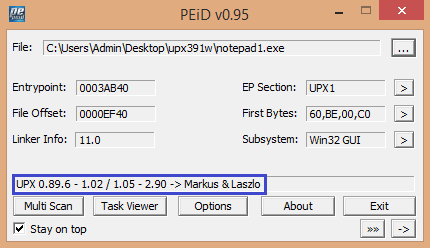
\includegraphics[scale=0.9]{Figures/PEID.PNG}
\caption{Le programme PEiD}
\label{fig :PEID} 
\end{center}
\end{figure}
On remarque que PEiD a identifié le fichier comme étant packé avec UPX Version 0.89.6-1.02 ou de 1.05 à 2.90.
\newpage
\section{Conclusion}
Le format PE (Portable Executable, exécutable portable) est le format des fichiers exécutables et bibliothèques pour les systèmes d'exploitation Microsoft Windows : .exe (programmes), .ocx (OLE et ActiveX), .dll et .cpl (élément du panneau de configuration Windows). C'est un format dérivé du COFF.\\


Un fichier exécutable PE est structuré d'en- MZ-DOS, segment DOS, en-tête PE et la table des sections. Le PE Loader est un élément de Microsoft Windows permettant de reconnaître et de charger en mémoire des fichiers PE. \\
Un Packer est un utilitaire dont le but est de compresser un programme afin de réduire sa taille initiale, tout en conservant son aspect exécutable.\\

Dans le chapitre suivant, on va présenter une conception de notre antivirus ainsi la conception de parseur de PE.
